\documentclass{standalone}

\usepackage{tikz}
\usepackage{standalone}
\usetikzlibrary{calc}

\begin{document}

    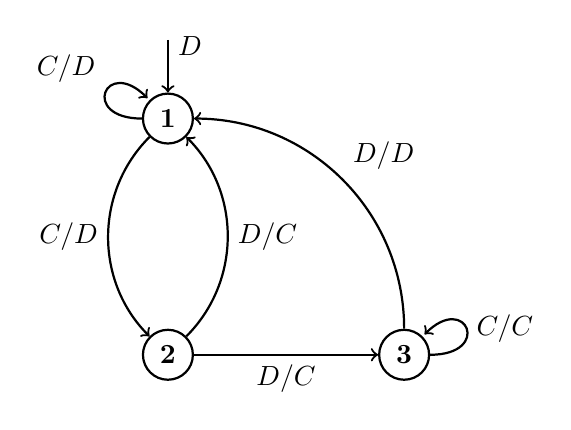
\begin{tikzpicture}

    \tikzstyle{state}=[minimum width=0.5cm, font=\boldmath];

    \node[circle, draw=black, thick]  (1) at (0,0) [state] {$1$};
    \node[circle, draw=black, thick] (2) at ($(1)+(0,-3)$) [state] {$2$}; 
    \node[circle, draw=black, thick]  (3) at ($(2)+(3,0)$) [state] {$3$};

    \coordinate[above of=1] (s);

    \draw (s) edge[out=-90, in=90, ->, thick] node [above right] {$D$} (1);

    \draw (1) edge[out=180, in=135, loop, thick] node [above left] {$C/D$} (1);
    \draw (3) edge[out=0, in=45, loop, thick] node [right] {$C/C$} (3);

    \draw (1) edge[out=-135, in=135, ->, thick] node [left] {$C/D$} (2);
    \draw (2) edge[out=45,in=-45,->,thick] node [right] {$D/C$} (1);
    \draw (2) edge[out=0,in=180,->,thick] node [below] {$D/C$} (3);
    \draw (3) edge[out=90,in=0,->,thick] node [above right] {$D/D$} (1);
    \end{tikzpicture}

\end{document}